\documentclass[landscape]{article}
\usepackage{amssymb}
\usepackage[landscape]{geometry}
\usepackage{color}
\usepackage{graphicx}
\usepackage{tikz}
\usepackage{amsfonts, amstext, amsmath}
\usepackage{wrapfig}
\usepackage{float}
\usepackage[export]{adjustbox}
\usepackage{tcolorbox}
\usepackage{times}
\usepackage{anyfontsize}
\usepackage{tikz}
\usepackage{graphicx}
\usepackage{multicol}
\usetikzlibrary{calc,bayesnet,shapes.geometric,arrows,chains,matrix,positioning,scopes,calendar,decorations.markings,decorations.pathreplacing,intersections}
\usetikzlibrary{arrows.meta}

\makeatletter
\tikzset{join/.code=\tikzset{after node path={%
      \ifx\tikzchainprevious\pgfutil@empty\else(\tikzchainprevious)%
      edge[every join]#1(\tikzchaincurrent)\fi}}
}
%\tikzset{>=stealth',every on chain/.append style={join},
%  every join/.style={->}
%}

\newcommand{\inputTikZ}[2]{%  
     \scalebox{#1}{\input{#2}}  
}

\newtcolorbox{mybox}{boxrule=6pt}

\def\argmax{\qopname\relax n{argmax}}
\def\s{\mathbf s}
\def\x{\mathbf x}
\def\u{\mathbf u}
\def\y{\mathbf y}
\def\d{\mathbf d}
\def\boldzero{\mathbf 0}
\def\pibold{\mbox{\boldmath $\pi$}}
\newcommand{\normal}[2]{\ensuremath{\mathcal{N}\left(#1,#2\right)}}
\newcommand{\given}{\mid}

\newenvironment{itemizeNoSymbol}{%
\renewcommand{\labelitemi}{}\begin{itemize}
\setlength{\itemsep}{1pt}
\setlength{\parskip}{0pt}
\setlength{\parsep}{0pt}}{\end{itemize}}


% set horizontal margins to center text (using current paperwidth &
% textwidth)
\newcommand{\equalmargins} {
\setlength{\oddsidemargin}{\paperwidth}
\addtolength{\oddsidemargin}{-\textwidth}
\setlength{\oddsidemargin}{0.5 \oddsidemargin}
\addtolength{\oddsidemargin}{-1in}
}

\setlength{\evensidemargin}{\oddsidemargin}

\renewcommand{\familydefault}{\sfdefault}

\input posterfonts.tex

% setup large (poster-sized) sheet
\setlength{\paperwidth}{841mm}
\setlength{\paperheight}{1189mm}
%\pdfpagewidth\paperwidth
%\pdfpageheight\paperheight
 
\setlength{\textwidth}{820mm}
\setlength{\textheight}{1170mm}
\setlength{\topmargin}{-.25truein}
 
\equalmargins
\setlength{\headsep}{0pt}
\setlength{\headheight}{0pt}

\pagestyle{empty}
\setlength{\parindent}{0mm}
\setlength{\parskip}{16pt}

% header style: title followed by a column-wide rule
\newcommand{\mysection}[1]{{\color[rgb]{.6,0,0}{\section*{{\LARGE #1}
        {\leaders\hrule height .2ex\hfill\kern0pt}}}}}

\begin{document}
\color{black}

% invisible rule is useful for spacing
\hrule width 0pt depth 0pt height 1pt

\begin{center}
  \HUGE
Approximating exponential family models \\ (not single distributions) with a two-network architecture \\
  \huge %
  Sean R. Bittner$^{1}$, John P. Cunningham$^2$ \\
  \LARGE
  $^{1}$Department of Neuroscience and $^{2}$Department of Statistics, Columbia University Medical Center
\end{center}

\begin{tikzpicture}[remember picture,overlay]
  \node[anchor=north east,inner sep=0pt, scale=0.35] at ($(current page.north east)+(+2.5cm,-1cm)$) {
     
\includegraphics{figs/CU_logo}
  };
\end{tikzpicture}

%%%%%%%%%%%%%%%%%%%%%%%%%%%%%%
\begin{minipage}[c]{0.28\linewidth}

\mysection{Motivation}
\large
\begin{itemize}
\item Many models used in machine learning are intractable exponential families.
\item Variational inference (VI) on intractable exponential families incurs a cost of optimization.
\item We introduce a deep generative two-network architecture called exponential family networks (EFNs) for learning intractable exponential family \textit{models} (not single distributions).
\item EFNs learn a smooth function $f_{\phi^*} : H \rightarrow \Theta$ mapping natty p's $\eta$ (i.e. \includegraphics[scale=0.2]{nattylight.png}) to optimal variational parameters $\theta^*$.
\begin{center}
\hspace{-1.0in}
\includegraphics[scale=1.0]{figs/amortizedVI/amortizedVI2.png}
\end{center}
\item EFNs afford substantial computational savings through amortized VI.
\end{itemize}

\mysection{Exp fams as target models $\mathcal{P}$}
\begin{itemize}
\item Exponential family models $\mathcal{P}$ have the form
\[\mathcal{P} = \left\{ \frac{h(\cdot)}{A(\eta)} \exp\left\{ \eta^\top t(\cdot) \right \} : \eta \in H \right\}\]
with natural parameter $\eta$, sufficient statistics $t(\cdot)$, base measure $h(\cdot)$, and log normalizer $A(\eta)$.\vspace{-1.0in}

\begin{minipage}[c]{0.7\linewidth}
\item We focus on the fundamental problem setup of probabilistic inference: $N$ conditionally independent observations $x_i$ given latent variable $z$.
\end{minipage}
\hspace{-0.2in}
\begin{minipage}[l]{0.25 \linewidth}
\vspace{1.5in}
\inputTikZ{0.5}{figs/fig1/fig1a_basic.tex} 
\end{minipage}
\item With exponential family prior and likelihood,
\[p_0(z) = \frac{1}{A_0(\alpha)} \exp\left\{ \alpha^\top t_0(z) \right\} \]
\[p(x_i|z) = \frac{1}{A(z)} \exp\left\{ \nu(z)^\top t(x_i) \right \} \]
\vspace{0.5cm} \\
our posterior is the following exp fam
\[p(z | x_1,...,x_N)  \propto  \exp\left\{ \begin{bmatrix} \alpha \\ \sum_i t(x_i) \\ -N \end{bmatrix}^\top\begin{bmatrix} t_0(z) \\ \nu(z) \\ \log A(z) \end{bmatrix} \right\}\]
which is intractable for nonconjugate priors, requiring computation for inference.

\end{itemize}


\mysection{Deep approximating families $\mathcal{M}$}
\begin{itemize}
\item Deep generative models are commonly used as approximating famillies to single distributions.
\item The density network (vertical) of our two-network architecture is a cascade of normalizing flows, which maps a base random variable $\omega$ to sample $z = g_\theta(\omega)$ with variational parameters $\theta$.
\[\omega \sim q_0(\omega), z = g_\theta(\omega) = g_L \circ ... \circ g_{1}(\omega)\] 
\item Bijective normalizing flows allow us to calculate the density for each sample.
\[ q_\theta(z) = q_0\left( g_1^{-1} \circ ... \circ g_L^{-1}(z) \right) \prod_{\ell=1}^L \frac{1}{| J^\ell_\theta(z) |} \]
\item The density network induces a model
\[\mathcal{M} = \left\{q(g_\theta(\omega)) : \theta \in \Theta \right\} \]
\end{itemize}


\end{minipage}
\hspace{1cm} \begin{minipage}[c]{0.4\linewidth}
%%%%%%%%%%%%%%%%%%%%%%%%%%%%%%
\mysection{Exponential family networks (EFNs)}
\large
\begin{mybox}
\begin{itemize}
\item EFNs are comprised of two networks :
\begin{itemize}
\item density network: $z = g_\theta(\omega)$
\item parameter network: $\theta = f_\phi(\eta)$
\end{itemize}
\item The parameter network (horizontal) is a fully connected neural network mapping $f_{\phi} : H \rightarrow \Theta$.
\item EFNs learn approximations $\mathcal{Q_\phi} \subset \mathcal{M}$ of exponential family models $\mathcal{P}$, so that $\mathcal{Q_\phi} \approx \mathcal{P}$, where $Q_\phi = \left\{q_{f_\phi} (z; \eta) : \eta \in H \right\}$.
\end{itemize}
\begin{center}
 \inputTikZ{0.5}{figs/fig1/fig1c.tex} 
 \end{center}
 \large
 \begin{itemize}
\item For a given $\eta$, we minimize the KL divergence $\mathcal{D}$ between the indexed distribution of $\mathcal{P}$ and $\mathcal{Q}_\phi$.
\[ D\left( q_\phi(z;\eta) || p(z;\eta) \right) = \mathbb{E}_{q_\phi} \Bigg( \log q_\phi(z;\eta) - \eta^\top t(z) + \log(A(\eta)) \Bigg) \]
We do this over a desired prior distribution $p(\eta)$,
\[\!\arg\!\min_{\!\!\!\!\!\!\!\!\!\!\!\phi} \mathbb{E}_{p(\eta)} \left( D\left( q_\phi(z;\eta) || p(z;\eta) \right)\right) \\ =  \!\arg\!\min_{\!\!\!\!\!\!\!\!\!\!\!\phi}  D\left( q_\phi(z;\eta)p(\eta) || p(z;\eta)p(\eta) \right)\]
which corresponds to the loss below.
\[ \mathbb{L}(\phi) = \frac{1}{K}\frac{1}{M}\sum_{k=1}^K \sum_{m=1}^M \bigg( \log q_0\left( g_{\theta^k}^{-1}\left(z^m\right)\right) + \sum_{\ell=1}^L  \log | J^\ell_{\theta^k}\left(z^m\right) | - \eta_k^\top t\left(z^m\right) \bigg) \] \\
 \end{itemize}
 \end{mybox} 
 
 \mysection{Intractable exponential families}
 \large
\begin{itemize}
\item Nonconjugate priors yield intractable exponential families requiring computation for inference.
\vspace{0.5in}
\end{itemize}
{\bf \Large Example: Hierarchical Dirichlet} \\ \\
\begin{minipage}[c]{0.325\linewidth}
\begin{itemize}
\item Dirichlet prior: \\
$z \sim Dir(\alpha)$ \\

\item iid Dirichlet draws: \\
$x_i \mid z \sim Dir(\beta z)$ \\ \\
\end{itemize}
\end{minipage}
\begin{minipage}[l]{0.25 \linewidth}
\vspace{-.2in}
\begin{center}
\hspace{-2.6in} \inputTikZ{0.5}{figs/fig1/HiDir.tex} 
 \end{center}
 \end{minipage}
 \hspace{-2in}
 \begin{minipage}[l]{0.425\linewidth}
 \vspace{-0.5in}
$p(z \mid X) \propto \exp \left\{ \eta^T t(z) \right\}$ \\ \\
 {\fontsize{22.44}{28.0}\selectfont $= \exp\left\{ \begin{bmatrix} \alpha - 1 \\ \sum_i \log(x_i) \\ -N \end{bmatrix}^\top\begin{bmatrix} \log(z) \\ \beta z \\ \log ( B( \beta a)) \end{bmatrix} \right\} $}  
 \end{minipage}
  \begin{minipage}[l]{0.4\linewidth}
 \begin{itemize}
 \item \vspace{-1.0in}Consider a situation in which we want to do inference on the hierarchical Dirichlet model for three seprate data sets (red dots, middle triangles) given a constant prior (top triangle).
 \end{itemize}
 \end{minipage}
 \begin{minipage}[l]{0.55\linewidth}
\begin{center}
\vspace{-0.5in} \inputTikZ{2.5}{figs/fig1/fig1b.tex} 
\end{center}
\end{minipage}
\begin{itemize}
\item Rather than running variational inference independently for each dataset, with an EFN, we can
\begin{enumerate}
\item Compute $\eta = \begin{bmatrix} \alpha - 1 \\ \sum_i \log(x_i) \\ -N \end{bmatrix}$ for each dataset.
\item Compute $\theta = f_{\phi^*}(\eta)$ using the parameter network. \\
\item Sample from the posterior using density network $z = g_{f_\phi^*(\eta)}(\omega)$ \\ (bottom triangles). \\
\end{enumerate}
\item By training an EFN for the hierarchical Dirichlet intractable exponential family, we are amortizing variational inference.
\end{itemize}
\end{minipage}
\hspace{1cm} \begin{minipage}[c]{0.28\linewidth}
%%%%%%%%%%%%%%%%%%%%%%%%%%%%%%
\mysection{Scaling dimensionality}
\large
\begin{itemize}
\item EFN scales to 40-50 dimensions for ground truth exponential families.
\end{itemize}
\begin{center}
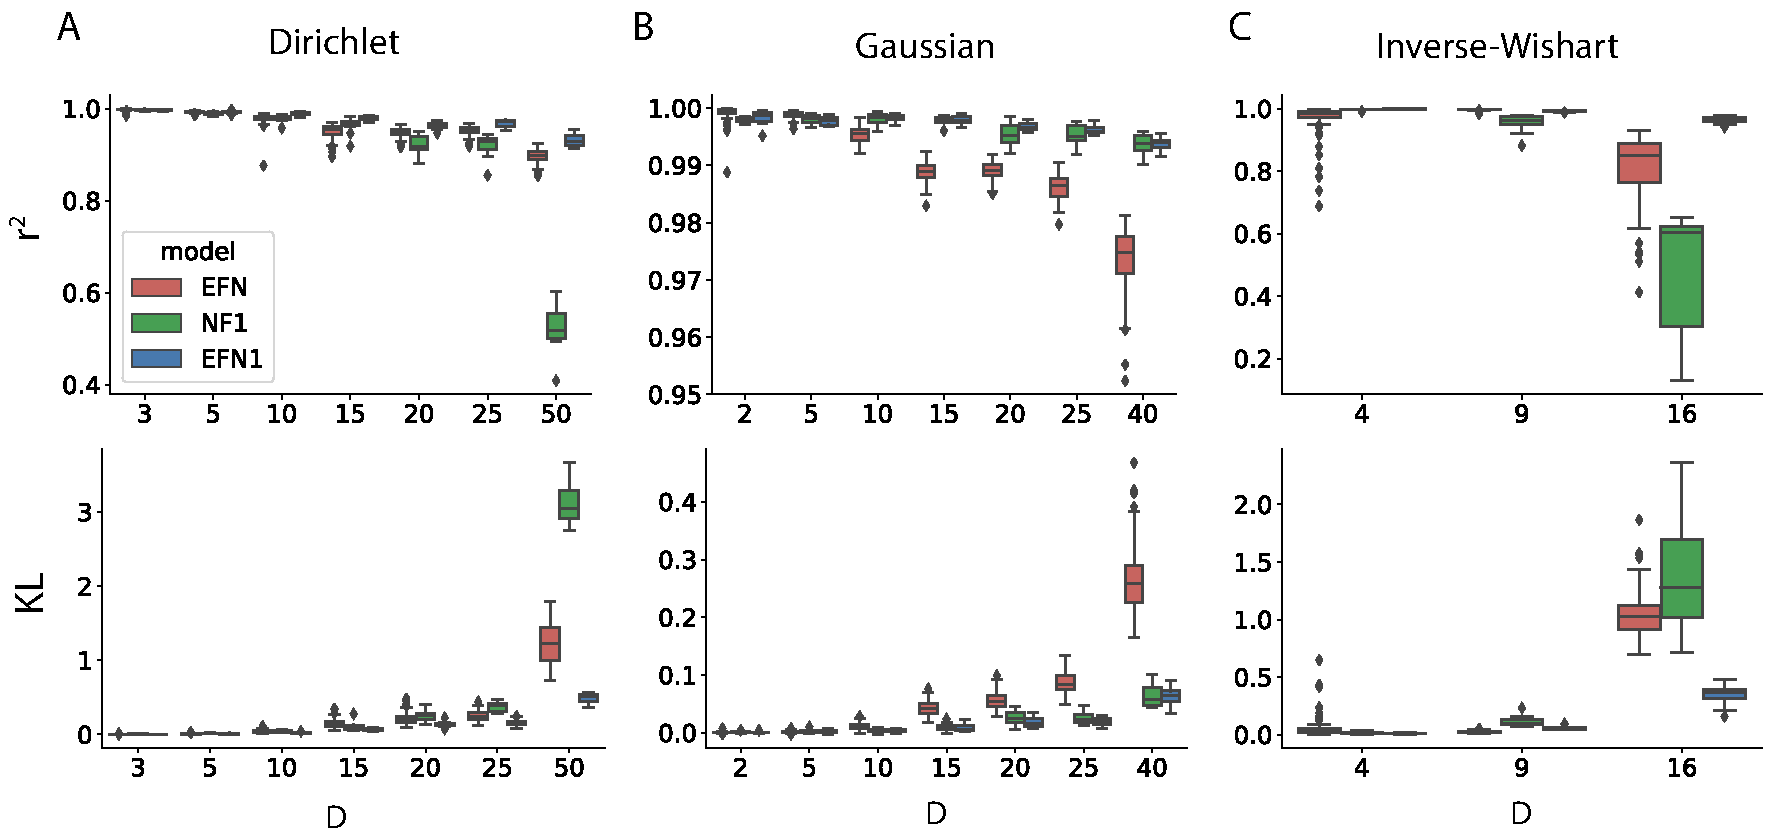
\includegraphics[scale=1.1]{figs/fig3/fig3.png}
\end{center}
\begin{itemize}
\item The regularization afforded by learning in a restricted model class $\mathcal{Q_\phi}$,results in better Dirichlet approximations in high dimensions.
\end{itemize}

\mysection{Lookup posterior inference with neural data}
\begin{itemize}
\item The log-Gaussian Poisson model is a popular intractable exponential family model used in neuroscience to represent neural spike emissions over a trial. 
\item If we want to run inference on the 2,964 datasets of 6.25Hz drift grating responses from [1], we can save a tremendous amount of computation using EFN (red) compared to independent runs of VI (blue).
\end{itemize}
\begin{center}
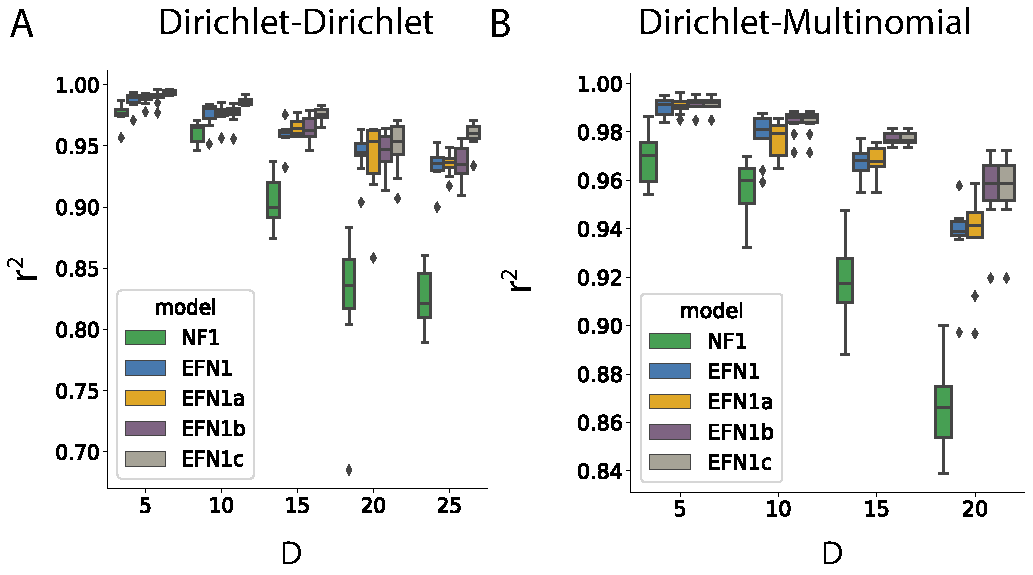
\includegraphics[scale=1.2]{figs/fig4/fig4.png}
\end{center}

\mysection{Summary}
\begin{itemize}
\item We learn exponential family models using a deep generative network, the parameters of which are the image of the natural parameters under another deep neural network. 
\item We demonstrated high quality empirical performance across a range of dimensionalities with the potential for better approximations when learning in a restricted model space.
\item Finally, we show computational savings afforded by immediate posterior inference lookup. \\
\end{itemize} 
\large

{\bf\Large References}
1. Smith, Matthew A., and Adam Kohn. ``Spatial and temporal scales of neuronal correlation in primary visual cortex." Journal of Neuroscience 28.48 (2008): 12591-12603. \\

{\bf\Large Acknowledgements} \\
NSF Graduate Research Fellowship,  DGE-1644869, McKnight Endowment Fund, NIH NINDS 5R01NS100066, Simons Foundation 542963, NSF 1707398, The Gatsby Charitable Foundation \\

\end{minipage}
\end{document}
